%projekt inżynierski - wersja do druku
%
%Przykładowy plik ułatwiający złożenie projektu dyplomowego inżynierskiego.
%UWAGA: Generowany napis na stronie tytułowej o treści PROJEKT DYPLOMOWY INŻYNIERSKI został zaproponowany przeze mnie i nie jest, póki co, potwierdzony przez władze wydziału. Przed ostatecznym oddaniem tak złożonej pracy należy upewnić się jaka powinna być treść tego napisu. W momencie gdy uzyskam informację na temat treści tego napisu, dokonam niezbędnych zmian w źródłach.

\documentclass[printmode,oneside]{mgr}
%\documentclass[eng,printmode,oneside]{mgr}
%opcje klasy dokumentu mgr.cls zostały opisane w dołączonej instrukcji

%poniżej deklaracje użycia pakietów, usunąć to co jest niepotrzebne
\usepackage{polski} %przydatne podczas składania dokumentów w j. polskim
%\usepackage[polish]{babel} %alternatywnie do pakietu polski, wybrać jeden z nich
\usepackage[utf8]{inputenc} %kodowanie znaków, zależne od systemu
\usepackage[T1]{fontenc} %poprawne składanie polskich czcionek

%pakiety do grafiki
\usepackage{graphicx}
\usepackage{subfigure}
\usepackage{psfrag}

%pakiety dodające dużo dodatkowych poleceń matematycznych
\usepackage{amsmath}
\usepackage{amsfonts}

%pakiety wspomagające i poprawiające składanie tabel
\usepackage{supertabular}
\usepackage{array}
\usepackage{tabularx}
\usepackage{hhline}

%do algorytmów
\usepackage[boxruled,longend,linesnumbered]{algorithm2e}
%%% this is from the \DeclareOptions part
\renewcommand{\listalgorithmcfname}{Lista algorytmów}%
\renewcommand{\algorithmcfname}{Algorytm}%
\renewcommand{\algorithmautorefname}{algorytm}%
\renewcommand{\algorithmcflinename}{linia}%
\renewcommand{\procedureautorefname}{procedura}%
\renewcommand{\functionautorefname}{funkcja}%

% do fragmentów kodu
\usepackage{listings}
\usepackage{color}
\definecolor{dkgreen}{rgb}{0,0.6,0}
\definecolor{gray}{rgb}{0.5,0.5,0.5}
\definecolor{mauve}{rgb}{0.58,0,0.82}
\lstset{frame=tb,
  language=Java,
  inputencoding=utf8,
  extendedchars=\true
  aboveskip=3mm,
  belowskip=3mm,
  showstringspaces=false,
  columns=flexible,
  basicstyle={\small\ttfamily},
  numbers=none,
  numberstyle=\tiny\color{gray},
  keywordstyle=\color{blue},
  commentstyle=\color{dkgreen},
  stringstyle=\color{mauve},
  breaklines=true,
  breakatwhitespace=true,
  tabsize=2
}

%do cytowania url
\usepackage{url}

%do dodatków na końcu
\usepackage[titletoc]{appendix}
%http://tex.stackexchange.com/questions/129807/how-can-i-rename-appendices-in-the-table-of-contents-and-in-the-text
%\renewcommand\appendixtocname{Dodatki}

%pakiet wypisujący na marginesie etykiety równań i rysunków zdefiniowanych przez \label{}, chcąc wygenerować finalną wersję dokumentu wystarczy usunąć poniższą linię
%\usepackage{showlabels}

%definicje własnych poleceń
\newcommand{\R}{I\!\!R} %symbol liczb rzeczywistych, działa tylko w trybie matematycznym
\newtheorem{theorem}{Twierdzenie}[section] %nowe otoczenie do składania twierdzeń

% http://tex.stackexchange.com/questions/7546/how-to-get-latex-symbol-in-document
\newcommand{\latex}{\LaTeX\ }
\newcommand{\tex}{\TeX\ }

%http://tex.stackexchange.com/questions/102792/create-table-with-only-header-bold-and-center
\newcommand*{\theader}[1]{\multicolumn{1}{|c|}{\bfseries #1}}

%dane do złożenia strony tytułowej
\title{Korygowanie harmonogramów\\ z uwzględnieniem awarii maszyn}
\engtitle{Re-scheduling with regard to machine failure}
\author{inż. Kamil Niemczyk}
\supervisor{dr hab. Wojciech Bożejko prof. nadzw. PWr}
%\guardian{dr hab. inż. Imię Nazwisko Prof. PWr, I-6} %nie używać jeśli opiekun jest tą samą osobą co prowadzący pracę

\date{2016} %standardowo u dołu strony tytułowej umieszczany jest bieżący rok, to polecenie pozwala wstawić dowolny rok

%poniżej jest lista kierunków i specjalności na wydziale elektroniki, należy wybrać właściwe lub dopisać jeśli nie ma odpowiednich
\field{Automatyka i Robotyka (AIR)}
\specialisation{Technologie informacyjne w systemach\\ automatyki (ART)}

%\usepackage[parfill]{parskip}
%tutaj zaczyna się właściwa treść dokumentu
\begin{document}

\bibliographystyle{plabbrv} %tylko gdy używamy BibTeXa, ustawia polski styl bibliografii

\maketitle %polecenie generujące stronę tytułową
%\dedication{6cm}{To jest przykładowa treść opcjonalnej dedykacji, należy ją zmienić lub usunąć w całości polecenie \texttt{$\backslash$dedication}- spokoKoles}
\cleardoublepage
\tableofcontents %spis treści
\cleardoublepage
%poniżej znajduje się przykładowa treść dalszej części dokumentu, zainteresowanych zachęcam do rozszyfrowania frazy "Lorem ipsum" :)
%
%
% TU ZACZYNA SIĘ WŁAŚCIWA TREŚĆ PRACY
%
%
\addcontentsline{toc}{chapter}{Wstęp}
\chapter*{Wstęp}
Problemy harmonogramowania, zdefiniowane pod koniec lat 70. XX wieku \cite{Garey76}, takie jak problem przepływowy, gniazdowy czy otwarty, klasyfikuje się jako NP trudne. Do ich rozwiązywania najczęściej stosuje się metaheurystyki takie jak Tabu Search, Symulowane Wyżarzanie, czy Algorytm Genetyczny.\\\\
W warunkach rzeczywistych, istnieje wiele rodzajów zakłóceń, których nie uwzględniają klasyczne problemy harmonogramowania. Powoduje to, że często nie wystarcza jednorazowe wyznaczenie harmonogramu dla określonego zestawu zadań, ponieważ w trakcie jego wykonywania warunki produkcji mogą ulec zmianie. Literatura opisuje różnego rodzaju zakłócenia: awarie/serwisowanie maszyn, niedokładna praca maszyn (ponowna obróbka elementu lub wykonanie zadania jeszcze raz), nadejście nowych zadań, anulowanie zadań, zmienny czas przetwarzania zadań, zmienny czas finalizacji zadań, a także ograniczony bufor transportu między stacjami roboczymi.\\\\
Okazuje się, że takie problemy można również rozwiązywać za pomocą wcześniej wspomnianych metaheurystyk odpowiednio przystosowując funkcję celu lub rozszerzając model danych o dodatkowe parametry. W pracy wzorowano się na podejściu harmonogramowania odpornego \cite{RFJSRMB_ElMekkawy11}, które oprócz minimalizacji całkowitego czasu wykonania harmonogramu $C_{max}$ (ang. \emph{makespan}) pozwala także zminimalizować jego podatność na opóźnienia wynikające z zakłóceń, takich jak awarie maszyn.  W przeciwieństwie do autorów \cite{RFJSRMB_ElMekkawy11} nie skorzystano z Algorytmu Genetycznego, a z \emph{TSAB} \cite{Smutnicki96} -- bardzo efektywnej odmiany Tabu Search odpowiednio przystosowując ją, aby uwzględniała możliwość awarii maszyn.\\\\
Uzyskane wyniki pozwoliły uzyskać dobre rezultaty niewielkim nakładem czasowym -- pojedencza instancja problemu obliczana jest średnio kilka sekund na współczesnym komputerze klasy PC. Nie oznacza to jednak końca badań w tej dziedzinie. Potencjał algorytmu \emph{TSAB} jest bardzo duży, dlatego kolejne wariacje zaproponowanego algorytmu pozwoliłyby w przyszłości na uzyskanie rozwiązań bliższych optimum w kontekście Elastycznych Problemów Gniazdowych.
%
\addcontentsline{toc}{chapter}{Cele i zakres pracy}
\chapter*{Cele i zakres pracy}
\section*{Cele pracy}
W pracy założono realizację celów wymienionych poniżej.
\begin{enumerate}
	\item Zbadanie dotychczasowych rozwiązań problemu korygowania harmonogramów w literaturze.
	\item Wybór oraz sformułowanie problemu harmonogramowania, który będzie analizowany w kontekście tematu pracy.
	\item Zaproponowanie algorytmu do rozwiązywania wybranego problemu harmonogramowania z uwzględnieniem awarii maszyn oraz jego opis tego rozwiązania.
	\item Stworzenie narzędzia służącego do wizualizacji wyników eksperymentalnych.
	\item Analiza wyników eksperymentalnych.
\end{enumerate}
\section*{Zakres pracy}
W rozdziale \ref{ch_lit_rev}. przeanalizowano dotychczasowe osiągnięcia w tematyce korygowania harmonogramów. Wydzielono w nim sekcje, które opisują różne podejścia w kontekście różnych zakłóceń, wymuszających potrzebę korygowania harmonogramów.\\\\
Rozdział \ref{ch_problem_def}. przedstawia sformułowanie wybranego problemu, który jest analizowany w~dalszej części pracy - Elastycznego Problemu Gniazdowego. Opisano w nim kryteria oraz ograniczenia, które wynikają ze specyfiki problemu.\\\\
Wybrane rozwiązania, czyli algorytmy, które zastosowano w badaniach opisano w rozdziale \ref{ch_algorithm}. Można tam znaleźć opis modelu danych, na którym operowano, strategii wyznaczania rozwiązania początkowego i w końcu głównego algorytmu oraz modyfikacji, które należy w nim wykonać, aby dostosować go do uwzględnienia awarii maszyn.\\\\
Ostatni, rozdział \ref{ch_experiments}. zawiera wyniki eksperymentów, które przeprowadzono z wykorzystaniem zaimplementowanych algorytmów.\\\\
Dodatek \ref{ch_code_snippets}. zawiera kod źródłowy stworzonej biblioteki, z której korzystano do generowania wykresów Gantt'a otrzymanych w rozdziale \ref{ch_experiments}. rozwiązań.
%
\chapter{Korygowanie harmonogramów z~uwzględnieniem zakłóceń \label{ch_lit_rev}}
Pierwsze próby rozwiązania problemu harmonogramowania zadań w procesach produkcyjnych sięgają końca lat 70 XX wieku \cite{Garey76}. Tak wcześnie jak zaczęto problemem się zajmować, wkrótce zakwalifikowano go jako problem NP trudny \cite{Garey76, Nawaz83}. Trzy ogólne problemy, które wydzielono w tym zagadnieniu, to:
\begin{itemize}
    \item problem przepływowy (flow shop),
    \item problem gniazdowy (job shop),
    \item problem otwarty (open shop).
\end{itemize}
Klasyfikacja problemów harmonogramowania jako NP trudne oznacza, że metody dokładne stosowane do rozwiązania tych problemów posiadają ponad-wielomianową złożoność obliczeniową, np. przegląd zupełny cechuje złożoność $O(n!)$. Z tego względu zaczęto stosować różnego rodzaju metaheurystyki, jak np. Tabu Search, Algorytm Genetyczny, czy Symulowane Wyżarzanie. W międzyczasie zaobserwowano, że w rzeczywistości procesom produkcyjnym towarzyszą różnego rodzaju zakłócenia, stąd rozpoczęto prowadzenie badań nad korygowaniem harmonogramów.
%
\section[Optymalizacja dyskretna oparta na uczeniu z nauczaniem]{Optymalizacja dyskretna oparta na uczeniu\\ z nauczaniem}
W \cite{DTLBO} autorzy proponują optymalizację dyskretną opartą na uczeniu z nauczaniem (\mbox{DTLBO}, ang. \emph{Discrete teaching-learning based optimization}) dla realistycznych problemów przepływowych. Uwzględniono tam jednoczesny wpływ 5 rodzajów zakłóceń:
\begin{itemize}
    \item awaria maszyny,
    \item nadejście nowego zadania,
    \item anulowanie zadań,
    \item zmienny czas przetwarzania zadań,
    \item zmienny czas finalizacji zadania (np. stygnięcie rozgrzanego elementu).
\end{itemize}
Odnośnie awarii maszyn, zakłada się tutaj, że nie wiemy kiedy występują, ani jak długo trwają. Ponadto, zadanie przerwane przez taką awarię, po jej usunięciu jest kontynuowane od momentu jego przerwania. W zależności od tego czy dana operacja została zakończona przed wystąpieniem awarii, przerwana przez awarię lub miała się dopiero wykonać, zostaje przypisana do odpowiedniej grupy. Wszystkie przerwane zadania pozostają na~swoich maszynach, a  kolejne zadania są przesuwane w czasie, w zależności od~oszacowania czasu naprawy usterki. W przypadku nadejścia nowego zadania stosuje się reaktywne procedury, które odpowiednio plasują je w harmonogramie. Poza sytuacjami wystąpienia zakłóceń nie jest dopuszczalne przerywanie zadań, a kolejne operacje danego zadania nie mogą się na siebie nakładać. Poza fazami nauczania i uczenia, charakterystycznymi dla TLBO wykorzystano tutaj również iteracyjny algorytm zachłanny (IG) w celu przyspieszenia procesu ewolucji. Celem porównania wybranej przez autorów metody w zależności od~jej parametryzacji, skonstruowano sześć wariantów TLBO, spośród których wyłoniono najlepszy i wykorzystano do konstrukcji kolejnych czterech wariantów DTLBO. Ponownie w~testach wybrano najwydajniejszy wariant i ostatecznie porównano go z algorytmami:
\begin{itemize}
    \item hGA - hybrydowy algorytm genetyczny,
    \item IG - iteracyjny algorytm zachłanny,
    \item ILS - iteracyjny algorytm poszukiwań lokalnych,
    \item PSO - optymalizacja rojem cząstek.
\end{itemize}
Wyniki zestawiono na podstawie testów na 90 instancjach Taillard'a z modelem zakłóceń zapożyczonym z \cite{Katragjini2013}. Jako kryterium porównawcze zastosowano względne odchylenie procentowe (\emph{RPD - Relative prcentage deviation}) od najlepszego wyniku dla danej instancji. Z~uwagi na wykorzystany w funkcji celu współczynnik kary, wyniki podzielono na 3 kategorie, w których współczynniki kary wynosiły odpowiednio 0.1, 0.5 oraz 0.9. We wszystkich przypadkach algorytm DTLBO pozwolił uzystać autorom najlepsze wyniki, niestety jednak kosztem znacząco wyższej złożoności obliczeniowej (średnie $RPD = 18,79$, podczas gdy ILS uzyskało wynik $RPD = 1,29$).
%
\section[Podejście ewolucyjne w harmonogramowaniu  proaktywnym]{Podejście ewolucyjne w harmonogramowaniu\\ proaktywnym}
Kolejna pozycja literaturowa \cite{KBEPS} rozważa harmonogramowanie proaktywne w odpowiedzi na losowe (stochastyczne) awarie maszyn w pogarszających się środowiskach produkcyjnych, gdzie właściwy czas przetwarzania zadania wydłuża się proporcjonalnie do~używania maszyny i jej wieku. Zaznacza się tu istotność odporności rozwiązania (ang. \emph{solution robustness}), z uwagi na obszary, których problem ten dotyka. Może być to sytuacja, kiedy firmy udostępniają przez Internet swoje harmonogramy produkcji swoim dostawcom surowców, aby dostawy mogły się odbywać w filozofii Just In Time. Ma to również znaczenie, jeśli chcieć posługiwać się tymi odpornymi rozwiązaniami problemu do budowy wskaźnika wydajności z punktu widzenia kierownictwa i operatorów hal produkcyjnych. \mbox{Co również} istotne, zasugerowano że umożliwiłyby one wgląd w niedaleką przyszłość pozwalając tym samym na sugerowanie konkurencyjnych terminów dostaw dla klientów. Podobnie jak w przypadku \cite{DTLBO}, tutaj również analizowano problem przepływowy, bez możliwości bezpośredniego przerywania zadań, gdzie awarie maszyn występują zgodnie z pewnym rozkładem prawdopodobieństwa, z tym że w tym artykule ustalany jest on na podstawie statystycznych danych historycznych. Co odróżnia tą publikację od poprzedniej, jest uwzględnienie stopniowego pogarszania czasu przetwarzania operacji z uwagi na czas pracy i wiek maszyny oraz fakt, że reakcja na awarię maszyny jest natychmiastowa, przerwane zadanie musi zostać wykonane jeszcze raz (od samego początku) oraz, jeśli chodzi o aspekt starzenia się maszyn, po naprawie wszystkie uszeregowane zadania na naprawionej maszynie wykonują się w oryginalnie założonym przedziale czasu, bez pogorszenia wynikającego z opisanych wyżej przyczyn. Głównym wyznacznikiem jakości zbudowanego algorytmu (autorzy nazwali go ADK/SA-NSGA-II) była analiza wariancji (ANOVA). Jako punkt odniesienia przyjęto wielokryterialny algorytm ewolucyjny (MOEA/D, ang. \emph{Multi objective evolutionary algorithm}). W rezultacie rozwiązanie autorów uzyskało znacząco lepszą zbieżność dla mniejszych instancji (30-200 zadań), jednak powyżej tego pułapu (300-500 zadań) przegrało z konkurentem.  
%
\section{Wyznaczanie harmonogramów od nowa}
Jeszcze inne podejście analizuje się w artykule \cite{EDSBCR}, gdzie proponuje się strategię sterowaną zdarzeniami, nie tyle korygując harmonogram, co za każdym razem tworząc go na nowo. Problem dotyczy harmonogramowania m identycznych równolegle pracujących maszyn z uwzględnieniem czasu przezbrojeń każdej z maszyn między wykonywanymi zadaniami przez pojedynczy serwer. W pracy podano definicję korygowania harmonogramów:
\begin{quotation}
\emph{,,Aktualizacja istniejącego harmonogramu produkcyjnego w odpowiedzi\\ na nieprzewidywalne zdarzenia czasu rzeczywistego, aby zminimalizować\\ ich wpływ na wydajność systemu.''}
\end{quotation}
Pytanie jakie należałoby sobie postawić to: ,,Jak i kiedy reagować na te zdarzenia czasu rzeczywistego?''. Odpowiedź nie jest jednoznaczna, co sugeruje też dalsza treść artykułu. Sugeruje się różne podejścia. Odnośnie tego ,,jak'' proponuje się naprawę harmonogramu, polegającą na pewnych lokalnych dopasowaniach, bądź też ustalenie harmonogramu zupełnie od nowa. Natomiast, jeśli spytać ,,kiedy'' reagować,  przedstawiane są trzy podejścia: periodyczne, polegające na korygowaniu cyklicznym, sterowane zdarzeniami, czyli korekty są wprowadzane tylko w sytuacji zarejestrowania określonych zdarzeń, oraz hybrydowe, będące połączeniem dwóch poprzednich.\\\\
Wracając do tematyki problemu przedstawionego w artykule, ponieważ zakłada się istnienie tylko jednego serwera, wydzielono trzy oszacowania czasu przezbrojenia maszyn:
\begin{description}
    \item[Mniejszy (\emph{minor})] -- kiedy maszyna będzie przetwarzać pierwsze zadanie na początku harmonogramu; jeśli awaria maszyny przerwała jakieś zadanie, tego typu przezbrojenie będzie również wymagane.
    \item[Średni (\emph{medium})] -- jeśli poprzednio wykonywane na maszynie zadanie jest tego samego typu co kolejne, które ma się wykonać na tej samej maszynie.
    \item[Większy (\emph{major})] -- w przypadku gdy kolejne zadanie do wykonania na tej samej maszynie różni się typem od zadania, które zostało na niej ukończone.
\end{description}
Dopuszcza się przerywanie zadań. Stochastyczną awaryjność maszyn określają dwa współczynniki o rozkładzie wykładniczym: średni czas między awariami (MTBF, ang. \emph{Mean Time Between Failure}) oraz średni czas do wykonania naprawy (MTTR, ang. \emph{Mean time to repair}). Z uwagi na fakt większej złożoności obliczeniowej podczas wyznaczania harmonogramu za każdym razem od nowa w porównaniu z korygowaniem harmonogramu, przyjęto strategię kolejkowania nadchodzących zadań i układania harmonogramu jedynie dla części z nich. Autorzy wydzielili cztery zdarzenia, które powodują uruchomienie procedury ustalenia nowego harmonogramu:
\begin{description}
    \item[Zdarzenie \#1: nadejście nowego zadania] -- w ten sposób system zapełnia pulę harmonogramowanych zadań aż do osiągnięcia zadanej górnej granicy liczby harmonogramowanych zadań.
    \item[Zdarzenie \#2: awaria maszyny] -- zadanie które zostało przerwane zostaje dodane do~puli zadań będących w harmonogramie i ustala się nowy harmonogram z pominięciem maszyny, która uległa awarii.
    \item[Zdarzenie \#3: naprawienie maszyny] -- ustala się nowy harmonogram dla zadań już uszeregowanych, ale których wykonywanie jeszcze się nie rozpoczęło - tym razem już z uwzględnieniem maszyny, która wcześniej uległa awarii.
    \item[Zdarzenie \#4] -- aktywuje się na koniec \textbf{zdarzenia \#1} oraz w momencie kiedy liczba zadań w puli tych już uszeregowanych na maszynach spada poniżej pewnej dolnej granicy. Powoduje uwolnienie z kolejki określonej liczby zadań i dodanie do zadań będących w puli już uszeregowanych zadań oraz wyznaczenie nowego harmonogramu.
\end{description}
Układanie harmonogramu wyzwolone każdym z powyższych zdarzeń uwzględnia jedynie maszyny, które są dostępne (mogą pracować). W przypadku gdy choć jedna maszyna nie jest dostępna (np. na skutek awarii) harmonogram nie zostaje wyznaczony. Schemat dodawania zadań z kolejki do ułożenia harmonogramu pokazano na rysunku \ref{rys_kolejkowanie_na_serwerze}.
\begin{figure}[!ht]
\begin{center}
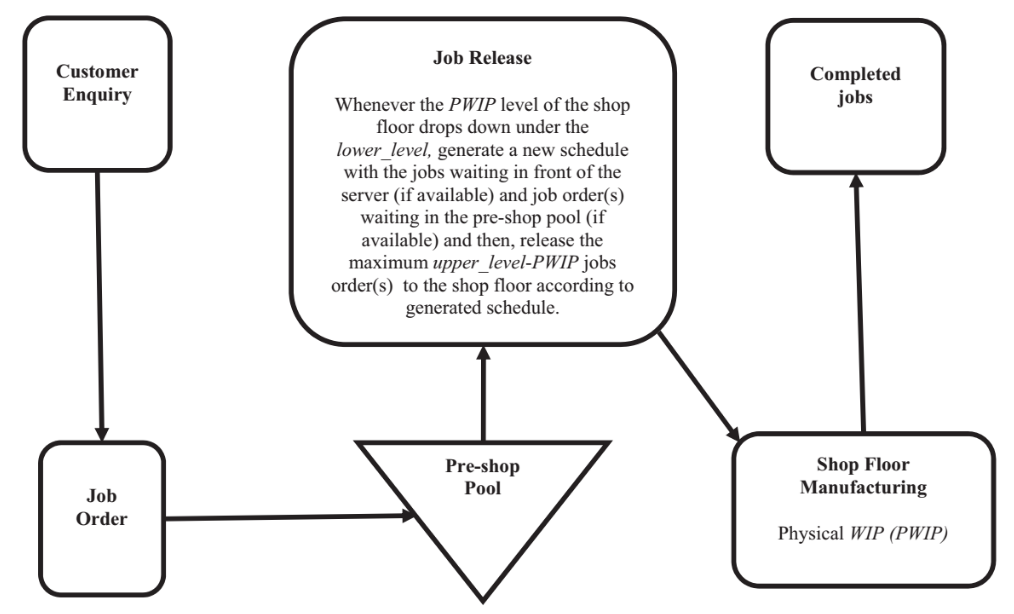
\includegraphics[scale=1.0,width=16cm]{rysunki/kolejkowanie_na_serwerze.png}
\caption[Schemat kolejkowania nadchodzących zadań oraz dodawanie ich do puli zadań, dla których zostaje wyznaczony nowy harmonogram]{Schemat kolejkowania nadchodzących zadań oraz dodawanie ich do puli zadań, dla których zostaje wyznaczony nowy harmonogram. Na diagramie za kolejnością strzałek: klient składa ofertę, pula wszystkich zadań, kolejka zadań oczekujących na dodanie do puli zadań w harmonogramie, wyzwolenie zadań (zdarzenie \#4), fizyczne wykonywanie zadań na hali produkcyjnej, wykonane zadania. Źródło: \protect\cite{EDSBCR}}
\label{rys_kolejkowanie_na_serwerze}
\end{center}
\end{figure}
Z wykorzystaniem algorytmu symulowanego wyżarzania (SA) oraz reguł planowania przydziału procesora (DR, ang. \emph{Dispatching Rules}), takich jak SPT, LPT oraz FIFO, wykonano symulacje dla proponowanego rozwiązania przedstawionego problemu. Przyjęto, że:
\begin{itemize}
    \item na hali produkcyjnej pracuje równolegle 10 identycznych maszyn,
    \item istnieje 50 różnych typów zadań,
    \item czas przetwarzania każdego zadania mieści się w zakresie 100-500,
    \item \textbf{większe} czasy przezbrojenia mieszczą się w zakresie 20-100,
    \item \textbf{średnie} czasy przezbrojenia wynoszą 10,
    \item \textbf{mniejsze} czasy przezbrojenia wynoszą 5,
    \item wartość średnia rozkładu wykładniczego dla MTBF wynosi 12000,
    \item wartość średnia rozkładu wykładniczego dla MTTR wynosi 3000.
\end{itemize}
Ostatecznie, na podstawie przeprowadzonych eksperymentów, wywnioskowano, że algorytm symulowanego wyżarzania osiągnął lepsze rezultaty niż FIFO, LPT czy SPT.
%
\section[Analiza wydajności linii produkcyjnych ze skończonym buforem]{Analiza wydajności linii produkcyjnych\\ ze skończonym buforem}
Pozycja \cite{MSTAWFB} pokazuje jeszcze inny problem produkcyjny związany z awarią maszyn. Analizuje się tutaj wydajność linii produkcyjnej składającej się z dwóch stacji roboczych połączonych wspólnym buforem o skończonej pojemności, gdzie na każdą ze stacji składają się równolegle niezależnie pracujące maszyny. Ilustracja problemu została przedstawiona na Rysunku \ref{rys_bufor}.
\begin{figure}[!ht]
\begin{center}
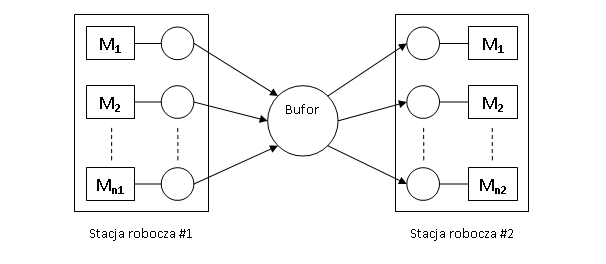
\includegraphics[scale=1.0,width=16cm]{rysunki/bufor.png}
\caption{Poglądowy schemat analizowanej w pracy \cite{MSTAWFB} linii produkcyjnej.}
\label{rys_bufor}
\end{center}
\end{figure}\\
Artykuł opisuje możliwe stany każdej z maszyn, których możliwe stany przedstawiono poniżej:
\begin{description}
    \item[Pracuje (\emph{working})]-- czyli obrabia pewien element,
    \item[Jest zagłodzona (\emph{starving})]-- w sytuacji gdy bufor przed stacją roboczą nie zawiera dostępnych do obróbki elementów,
    \item[Jest zablokowana (\emph{blocked})]-- jeżeli skończyła obróbkę elementu, ale bufor za stacją roboczą jest pełny.
\end{description}
Odnośnie awaryjności maszyn, w pracy zakłada się, że tylko pracująca maszyna może ulec awarii, a zagłodzona lub zablokowana już nie. Dodatkowo, czego nie uwzględniono na powyższym schemacie, przed stacją roboczą \#1 oraz za \#2, istnieją bufory o nieskończonych pojemnościach. Autorzy porównali zaproponowany trójstanowy model maszyn z modelem dwustanowym, który opracowali Diamantidis i Papadopoulos w \cite{Diamantidis2009}, oraz z modelem symulacyjnym WITNESS. Model trójstanowy okazał się dawać rezultaty bardzo zbliżone jakościowo do wyników działania na modelu symulacyjnego - miejscami nawet lepsze.
%
\section{Potrzeba ponownej obróbki elementów}
Co zostało już zaznaczone we wcześniej wspomnianych tytułach, również autorzy pracy \cite{IPMRWJRD} zauważyli inne przyczyny potrzeby korygowania harmonogramów. Poza tymi związanymi z zasobami (awarie lub zawieszanie się maszyn, przestoje lub blokady linii produkcyjnej, opóźnienia w dostawach, itp.) istnieją również takie, które mają związek z samymi zadaniami wykonywanymi na maszynach (anulowanie lub nadejście nowych zadań, zmiany ich priorytetów, czasów obróbki, czy też potrzeba poprawek lub przeróbek). W takich sytuacjach należy znaleźć kompromis między wydajnością (koszty harmonogramowania) a~stabilnością (koszty zakłóceń). Koszty zakłóceń typowo mierzy się badając jak często oraz w jakim stopniu zmieniają się: kolejność wykonywanych zadań, czasy rozpoczęcia oraz zakończenia zadań, a także obciążenie maszyn w poprzednim oraz nowym harmonogramie. Natomiast koszty  harmonogramowania wyrażają się bardzo prosto, w całkowitym czasie wykonania harmonogramu. Artykuł skoncentrował się nie tyle na metodach wyznaczania harmonogramów (zastosowano tu prostą metodę planistyczną SPT), co na samym zagadnieniu zakłóceń wynikających z potrzeby ponownej obróbki przetwarzanych na maszynach elementów.
%
\section{Harmonogramowanie odporne}
Artykuły \cite{RFJSRMB_ElMekkawy11} oraz \cite{RFJSRMB_Chen} poruszają interesujący temat alternatywnych rozwiązań w poszukiwaniu optymalnych harmonogramów. Odporne harmonogramowanie w problemach gniazdowych z uwzględnieniem losowych awarii maszyn \cite{RFJSRMB_ElMekkawy11} zostało tutaj zrealizowane z wykorzystaniem hybrydowego algorytmu genetycznego. Odporność algorytmu polega na tym, że generowane harmonogramy nie są tak ciasno upakowane, jak te które otrzymuje się szeregując zadania w podejściu statycznym. Dzięki temu awaria maszyny nie zawsze musi oznaczać opóźnienie całego harmonogramu. Widać to na Rysunkach \ref{rys_tradycyjny_jobshop} i \ref{rys_odporny_jobshop} W przypadku harmonogramowania statycznego (lewa strona na rysunkach) obydwa rozwiązania są~takie same. Jednak z punktu widzenia harmonogramowania dynamicznego (prawa strona na rysunkach), np. wiemy, że są duże szanse awarii maszyny M1, rozwiązanie przedstawione na rysunku \ref{rys_odporny_jobshop} jest lepsze pod względem odporności na nieplanowane opóźnienia pierwotnego harmonogramu.
\begin{figure}[!ht]
\begin{center}
\minipage{0.5\textwidth}
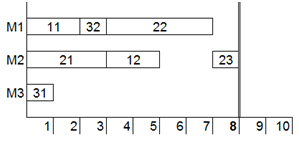
\includegraphics[width=1.0\linewidth]{rysunki/tradycyjny_jobshopA.png}
\endminipage \hfill
\minipage{0.5\textwidth}%
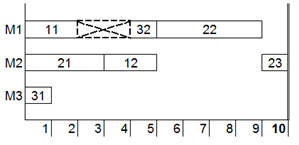
\includegraphics[width=1.0\linewidth]{rysunki/tradycyjny_jobshopB.png}
\endminipage
\caption[Tradycyjne harmonogramowanie]{Tradycyjne harmonogramowanie. Gęsto upakowane zadania usztywniają harmonogram. Awaria maszyny M1 w punkcie czasu 2 powoduje opóźnienie czasu wykonania harmonogramu.}
\label{rys_tradycyjny_jobshop}
\end{center}
\end{figure}
\begin{figure}[!ht]
\begin{center}
\minipage{0.5\textwidth}
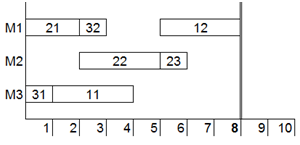
\includegraphics[width=1.0\linewidth]{rysunki/odporny_jobshopA.png}
\endminipage \hfill
\minipage{0.5\textwidth}%
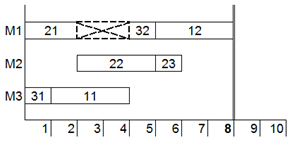
\includegraphics[width=1.0\linewidth]{rysunki/odporny_jobshopB.png}
\endminipage
\caption[Harmonogramowanie odporne]{Harmonogramowanie odporne. Luźno rozmieszczenie zadań pozwala na minimalne zmiany w harmonogramie oraz zachowanie czasu jego wykonania w przypadku awarii maszyny M1.}
\label{rys_odporny_jobshop}
\end{center}
\end{figure}
Proponowanym podejściem jest rozwiązanie elastycznego problemu gniazdowego za pomocą hybrydowego algorytmu genetycznego opracowanego przez autorów \cite{RFJSRMB_ElMekkawy11} w ich wcześniejszym artykule \cite{AEHGAFJS_ElMekkawy11}. Korzysta się z niego dwukrotnie - za pierwszym razem do stworzenia harmonogramu, który minimalizuje czas wykonania wszystkich zadań, tak jak w klasycznym elastycznym problemie gniazdowym, a następnie uruchamiany jest ponownie, w celu zwiększenia odporności harmonogramu na późniejsze zmiany (uwzględnienie możliwości awarii maszyn). Reprezentacja genów chromosomów to~trójki liczb $(k,i,j)$ oznaczające kolejno:
\begin{itemize}
    \item $k$ -- numer maszyny,
    \item $i$ -- numer zadania,
    \item $j$ -- numer operacji zadania $i$-tego.
\end{itemize}
Przykładowo: chromosom (2,1,1)-(1,2,1)-(1,1,2)-(2,2,2) oznacza, że na maszynie 1. wykonają się kolejno operacja 1. zadania 2. oraz operacja 2. zadania 1., a na maszynie 2. operacja 1. zadania 1. oraz operacja 2. zadania 2. Dzięki takiej reprezentacji oraz zastosowaniu w algorytmie odpowiednio zaprojektowanych operatorów krzyżowania i mutacji pozwalają zapobiec osiągnięciu zabronionych harmonogramów, co pozwoliło autorom pominąć etap walidacji chromosomów otrzymanych w wyniku wykorzystania tych operatorów. Przypadki testowe zostały zapożyczone z prac \cite{Kacem2002b,Mesghouni1997,LeeDiCesare1994,Kacem2002a,Brandimarte1993}. Oprócz analizy wariancji otrzymanych w eksperymentach populacji (ANOVA) zbadano również wydajność harmonogramu pod kątem stabilności i odporności oraz czasu wykonania wszystkich zadań (ang. \emph{makespan}).
\begin{center}***\\\end{center}
Potrzeba korygowania harmonogramów jest bardzo obszernie analizowana w literaturze. Proponowane metody to najczęściej poszechnie znane heurystyki, takie jak Tabu Search, Symulowane Wyżarzanie, Algorytm Genetyczny, czy Algorytm Ewolucyjny, sparametryzowane pod kątem konkretnych problemów. Trudno określić jednoznacznie, która z nich jest najlepsza.
%
%
%
\chapter{Sformułowanie problemu \label{ch_problem_def}}
Elastyczny Problem Gniazdowy (ang. \emph{Flexible Job Shop Problem}, \emph{FJSP}) jest uogólnieniem klasycznego Problemu Gniazdowego. Różnica poleta na tym, że nie uwzględnia się w~nim ograniczenia dotyczącego maszyny, która ma wykonać konkretną operację w zadaniu. W~konsekwencji, dla każdej z operacji w trakcie układania harmonogramu należy podjąć dodatkową decyzję o wyborze maszyny, która przetworzy daną operację. Ponieważ już klasyczny Problem Gniazdowy został zakwalifikowany do problemów silnie NP-trudnych, z uwagi na dodatkowe skomplikowanie FJSP także zakwalifikowano jako problem silnie NP-trudny \cite{Tay2004}. Sformułowanie problemu deterministycznego Elastycznego Problemu Gniazdowego podane w \cite{AEHGAFJS_ElMekkawy11} przedstawia się jak poniżej:
\begin{itemize}
    \item Mamy $n$ niezależnych wzajemnie zadań $J$ indeksowanych przez $i$.
    \item Wszystkie zadania są gotowe do rozpoczęcia przetwarzania w chwili czasu 0.
    Każde zadanie $J_i$ składa się z $O_i$ operacji, których kolejność wykonania jest określona przez $O_{ij}$, gdzie $j = 1, ..., O_i$.
    \item Mamy $m$ maszyn $M$ indeksowanych przez $k$.
    \item Maszyny nigdy nie ulegają awarii i są zawsze dostępne.
    \item Każda operacja $O_{ij}$ ma zdefiniowany zbiór maszyn $M_{kij} \subseteq {1, ..., m}$, które mogą ją~przetwarzać.
    \item Poszczególne czasy przetwarzania operacji $O_{ij}$ na maszynach $M_{kij}$ są zdefiniowane w zbiorze $P_{ij}$ o tym samym rozmiarze co $M_{kij}$ -- przetwarzanie na maszynie $k$ zdefiniowane jest przez $p_{ijk}$.
    \item Odpowiednio, jako czas rozpoczęcia uszeregowanej operacji oznacza się $S_{ij}$, a czas jej zakończenia $C_{ij}$ wyraża się przez sumę $S_{ij} + p_{ijk}$.
    \item Czasy przezbrojenia maszyn są niezależne od kolejności operacji na nich wykonywanych i wliczone są w ich czasy przetwarzania.
    \item Nie można przerywać przetwarzania operacji.
    \item Każda z maszyn może przetwarzać jednocześnie co najwyżej jedną operację.
    \item Ograniczenia kolejnościowe przetwarzania operacji w zadaniach może zostać zdefiniowane dla dowolnej pary operacji.
\end{itemize}
Celem jest minimalizacja całkowitego czasu wykonania harmonogramu $C_{max}$, w literaturze anglojęzycznej częściej określanym jako \emph{makespan}. Jendak w rzeczywistych warunkach produkcyjnych ustalony harmonogram może zostać zakłócony, na przykład na skutek awarii maszyny. Pozycja \cite{RFJSRMB_ElMekkawy11} zakłada pewną losowość występowania awarii maszyn. Jednak ta losowość jest zdeterminowana przez założenie posiadania historycznych danych ze środowiska produkcyjnego, a samo prawdopodobieństwo wystąpienia awarii jest wprost proporcjonalne do łącznego czasu pracy maszyny (suma czasów przetwarzania zakończonych operacji). Podobny efekt można uzyskać planując momenty wystąpienia awarii -- może to być na przykład zaplanowany serwis maszyny. W pracy zdecydowano się na zastosowanie tego drugiego podejścia. Dalszy jego opis można znaleźć w rozdziale \ref{ch_algorithm}.
%
\chapter{Opis algorytmów \label{ch_algorithm}}
Opracowany algorytm inspirowany jest interesującym podejściem harmonogramowania odpornego. Korzysta on z procedury wyznaczającej pierwszy harmonogram metodą wstawień dostosowaną do elastycznych problemów gniazdowych (\emph{IniPopGen}) zaproponowaną przez Al-Hinai oraz ElMekkawy w \cite{AEHGAFJS_ElMekkawy11}. Choć \emph{IniPopGen} zaprojektowano do działania z~algorytmem genetycznym, to praktycznie bez problemu udało się go zaadoptować do~wykorzystania z metodą Tabu Search z nawrotami (\emph{TSAB}), którą pierwszy raz opisano w~\cite{Smutnicki96}. Decyzję o rezygnacji z wykorzystania algorytmu genetycznego proponowanego przez autorów \emph{IniPopGen} podjęto z uwagi na wysoką złożoność obliczeniową metody. O ile dla małych problemów, rzędu kilkudziesięciu operacji nie było to problemem, to już przy jednej z najmniejszych instancji Taillard'a (225 operacji, 15x15) jedynie inicjalizacja populacji 500 osobników zajmowała minutę. Dla porównania, algorytm \emph{TSAB} wykonuje wszystkie obliczenia dla tej samej instancji średnio w sekundę. Jego szybkość spowodowana jest mocno ograniczonym sąsiedztwem w każdej iteracji -- brane są pod uwagę tylko takie ruchy, które mają szansę na skrócenie ścieżki krytycznej harmonogramu poprzez zamianę operacji w blokach krytycznych \cite{Grabowski86}. Widać to w eksperymentach -- w ciągu kilku minut otrzymano przybliżone rozwiązania kolejno wszystkich 80 instancji opublikowanych przez Taillard'a dla problemu gniazdowego. Szczegółowe wyniki eksperymentów opisano w rozdziale \ref{ch_experiments}. Zaprojektowany algorytm pozwala rozwiązywać instancje Elastycznego Problemu Gniazdowego oraz jego szczególnych odmian, takich jak klasyczny Problem Gniazdowy, czy Problem Przepływowy.
%
\section{Model danych}
Podstawowym elementem harmonogramu jest operacja. W tabeli \ref{table_operation} zestawiono jej cechy charakterystyczne.
\begin{table}[ht]
\renewcommand{\arraystretch}{1.5}
\begin{tabular}{|c|l|}
    \hline
    \textbf{PID} & numer zadania, którego elementem jest operacja\\
    \hline
    \textbf{ID} & numer kolejnościowy operacji w zadaniu \textbf{PID}\\
    \hline
    \textbf{M} & numer maszyny, do której aktualnie przyporządkowano operację\\
    \hline
    \textbf{S} & czas rozpoczęcia wykonywania operacji w harmonogramie\\
    \hline
    \textbf{P} & \multicolumn{1}{m{14.25cm}|}{mapa czasów przetwarzania operacji na poszczególnych maszynach, na których można przetwarzać daną operację}\\
    \hline
    \textbf{C} & czas zakończenia operacji na maszynie \textbf{M}\\
    \hline
    \textbf{B} & bufor czasowy (domyślnie $=0$, więcej na ten temat w sekcji \ref{ch_awarie})\\
    \hline
\end{tabular}
\renewcommand{\arraystretch}{1}
\caption{Elementy opisujące pojedynczą operację harmonogramu.}
\label{table_operation}
\end{table}
Kilka operacji o ustalonej kolejności wykonania tworzy zadanie. Z~programistycznego punktu widzenia, zadanie jest tablicą operacji. Strukturę diagramu Gantt'a opisują dwie listy sąsiedztwa. Pierwsza z nich $LS_M$ definiująca kolejność wykonania na maszynach o rozmiarze $m$, gdzie $m$ jest liczbą maszyn. Natomiast druga, $LS_Z$ będąca kompletną kopią wszystkich operacji o rozmiarze $n$, gdzie $n$ jest liczbą zadań, i opisuje kolejność wykonania operacji w każdym z poszczególnych zadań. Połączenie tych dwóch zestawów danych, opisujących harmonogram oraz zadania, pozwala wygodnie poruszać się po harmonogramie. Taka reprezentacja danych bardzo przypomina graf skierowany opisany przez Nowickiego i Smutnickiego w \cite{Smutnicki96}. Pozwala ona na łatwą konwersję harmonogramu do formatu HTML, dzięki czemu uzyskano interaktywną graficzną prezentację wyników. Więcej na ten temat opisano w rozdziale~\ref{ch_experiments}.
%
\section{Rozwiązanie początkowe}
W pierwszej kolejności z pliku wczytywana jest pojedyncza instancja problemu i zapisywana jest do listy sąsiedztwa zadań $LS_Z$. Następnie, $LS_M$ tworzona jest przy pomocy algorytmu \emph{IniPopGen}. Otrzymana w wyniku tej metody lista $LS_M$ jest w pełni deterministyczna. Oznacza to, że za każdym razem przy określonej kolejności wykonania zadań wylosowanej na początku algorytmu skutkuje identyczną listą $LS_M$. W opisie tego algorytmu pominięto jedynie kroki związane z genami i chromosomami, które w metodzie Tabu Search nie mają żadnego zastosowania. Nazwę zachowano, aby ułatwić identyfikację w odniesieniu do źródła, z którego pochodzi.
%
\section{Tabu Search z nawrotami}
Podstawowym elementem na którym bazuje algorytm \emph{TSAB} jest ścieżka krytyczna. Jest to taki ciąg operacji, że opóźnienie którejkolwiek z nich spowodowałoby opóźnienie całego harmonogramu. Harmonogramy w Problemach Gniazdowych mogą mieć więcej niż jedną ścieżkę krytyczną. Każda ścieżka krytyczna dzieli się na bloki \cite{Grabowski86} -- ciągi operacji wykonywanych bez odstępów czasowych na określonej maszynie.
\begin{figure}[!ht]
\begin{center}
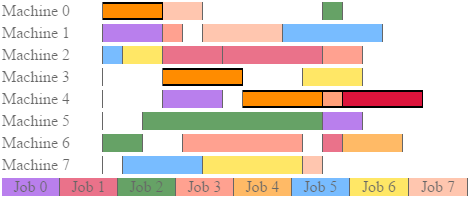
\includegraphics[scale=1.0]{rysunki/criticalPath2.png}
\caption[Przykładowy harmonogram wraz z wyróżnioną ścieżką krytyczną]{Przykładowy harmonogram wraz z wyróżnioną ścieżką krytyczną zawierającą dwa bloki krytyczne, każdy składający się z trzech operacji, na maszynach 1 i 4.}
\label{rys_critical_path_example}
\end{center}
\end{figure}
%
\begin{algorithm}[!ht]
    \SetKwInput{KwIn}{Przyjmuje}%
    \SetKwInput{KwOut}{Zwraca}%
    \SetKwInput{KwData}{Dane}%
    \SetKwInput{KwResult}{Wynik}%
    \SetKw{KwTo}{To}
    \SetKw{KwRet}{Zwraca}%
    \SetKw{Return}{Zwraca}%
    \SetKwBlock{Begin}{Początek}{Koniec}%
    \SetKwRepeat{Repeat}{Powtarzaj}{dopóki}%
    %
    \SetKwIF{If}{ElseIf}{Else}{Jeżeli}{to}{Przeciwnie, jeżeli}{Przeciwnie}{Koniec warunku}%
    %\SetKwSwitch{Switch}{Case}{Other}{switch}{do}{case}{otherwise}{end switch}%
    \SetKwFor{For}{Dla}{wykonaj}{Koniec pętli}%
    \SetKwFor{ForPar}{Dla}{wykonaj równolegle}{Koniec pętli}
    \SetKwFor{ForEach}{Dla każdego}{wykonaj}{Koniec pętli}%
    \SetKwFor{ForAll}{Dla wszystkich}{wykonaj}{Koniec pętli}%
    \SetKwFor{While}{Dopóki}{wykonuj}{Koniec pętli}%
    %
    Zainicjuj strukturę diagramu Gantt'a\;
    Wygeneruj losową kolejność wykonania zadań $J$ (np.: $J_2$, $J_1$, $J_3$)\;
    Ustaw $operCount = 1$ oraz $oper = 1$\;
    \While{ $(operCount \leq totNOper)$ }{
        \ForAll {zadań $i \in J$}{
            Znajdź wszystkie maszyny $M$, które mogą przetwarzać operację $O_{i,oper}$ (np. $M_1$, $M_3$)\;
            Wygeneruj tablicę czasów zakończenia $T$ operacji $O_{i,oper}$ o rozmiarze równym rozmiarowi $M$\;
            Zainicjuj $t_0$ i $t_1$\;
            \eIf {$O_{i,oper}$ jest pierwszą operacją}{
                Ustaw $t_0 = 0$\;
            }{
                Ustaw $t_0$ równe czasowi zakończenia przetwarzania poprzednika technologicznego $O_{i,oper-1}$\;
            }
            \ForAll {maszyn $k \in M$}{
                Zidentyfikuj czas przetwarzania $t_{i,oper,k}$ operacji $O_{i,oper}$ na maszynie $M_k$\;
                \eIf {$t_1 \leq t_0$}{
                    Ustaw $t_1 = 0$\;
                }{
                    Ustaw $t_0$ równe czasowi zakończenia przetwarzania ostatniej operacji na $M_k$\;
                }
                \uIf{$t_1 \leq t_0$}{
                    Dodaj $O_{i,oper}$ na $M_k$ z czasem rozpoczęcia $t_0$ i ustaw $T_{oper,k} = t_0 + t_{i,oper,k}$\;
                }
                \uElseIf{$t_{i,oper,k}$ zawiera się w przedziale czasu $[t_0 , t_1]$, czyli może być wykonane między uszeregowanymi już operacjami na $M_k$}{
                    Wstaw $O_{i,oper}$ na $M_k$ z możliwie najwcześniejszym czasem rozpoczęcia $t_s \geq t0$ oraz ustaw $T_{oper,k} = t_s + t_{i,oper,k}$\;
                }
                \Else{
                    Dodaj $O_{i,oper}$ na $M_k$ z czasem rozpoczęcia $t_1$ oraz ustaw $T_{oper,k} = t_1 + t_{i,oper,k}$\;
                }
            }
            Znajdź minimalny czas zakończenia w tablicy $T$ i przydziel $O_{i,oper}$ do odpowiadającej temu elementowi maszyny. Jeśli istnieje kilka maszyn, spełniające takie przyporządkowanie, należy wybrać pierwszą z nich\;
            ++operCount\;
        }
        ++oper\;
    }
    \caption{IniPopGen. Źródło: \cite{AEHGAFJS_ElMekkawy11}.}
\end{algorithm}
\ \\W algorytmie Tabu Search, aby był on jak najbardziej wydajny, najważniejsze jest obserwowane otoczenie (sąsiedztwo) bieżącego w danej iteracji rozwiązania oraz wybór najlepszego ruchu, który należy wykonać, aby przetransformować aktualne rozwiązanie do~tego wybranego. Za ten obszar w algorytmie \emph{TSAB} odpowiedzialny jest jest zmodyfikowany algorytm \emph{NSP} \cite{Smutnicki96}. Bazuje on na blokach krytycznych składających się z więcej niż jednej operacji. Do wygenerowania otoczenia wykonuje tylko takie ruchy, które polegają na zamianie kolejnością dwóch pierwszych lub dwóch ostatnich operacji w danym bloku. Pomija się jedynie sąsiadów, którzy mogliby zostać wygenerowani przez zamianę dwóch pierwszych operacji w pierwszym bloku ścieżki krytycznej oraz dwóch ostatnich w~ostatnim bloku krytycznym. Modyfikacja algorytmu polega na tym, że sprawdza się dopuszczalność wykonania danego ruchu, tzn. czy wykonanie ruchu nie naruszy ograniczeń kolejnościowych w jakimkolwiek zdaniu w harmonogramie. Pierwotnie, algorytm \emph{NSP} nie potrzebował takiego sprawdzenia, ponieważ nie był stosowany do Elastycznych Problemów Gniazdowych.
\begin{algorithm}[!ht]
    \SetKwInput{KwIn}{Przyjmuje}%
    \SetKwInput{KwOut}{Zwraca}%
    \SetKwInput{KwData}{Dane}%
    \SetKwInput{KwResult}{Wynik}%
    \SetKw{KwTo}{To}
    \SetKw{KwRet}{Zwraca}%
    \SetKw{Return}{Zwraca}%
    \SetKwBlock{Begin}{Początek}{Koniec}%
    \SetKwRepeat{Repeat}{Powtarzaj}{dopóki}%
    %
    \SetKwIF{If}{ElseIf}{Else}{Jeżeli}{to}{Przeciwnie, jeżeli}{Przeciwnie}{Koniec warunku}%
    %\SetKwSwitch{Switch}{Case}{Other}{switch}{do}{case}{otherwise}{end switch}%
    \SetKwFor{For}{Dla}{wykonaj}{Koniec pętli}%
    \SetKwFor{ForPar}{Dla}{wykonaj równolegle}{Koniec pętli}
    \SetKwFor{ForEach}{Dla każdego}{wykonaj}{Koniec pętli}%
    \SetKwFor{ForAll}{Dla wszystkich}{wykonaj}{Koniec pętli}%
    \SetKwFor{While}{Dopóki}{wykonuj}{Koniec pętli}%
    %
    \KwIn{Permutację $\pi$, zestaw możliwych ruchów $V(\pi) \neq \emptyset$, listę tabu $T$ oraz najkrótszy osiągnięty czas wykonania harmonogramu $C^*_{max}$.}
    \KwOut{Wybrany (najlepszy) ruch $v'$, powstałą przez wykonanie ruchu $v'$ permutację sąsiada $\pi'$ oraz zmodyfikowaną listę tabu $T'$.}
    Znajdź zestaw zakazanych ruchów, które poprawiają aktualne rozwiązanie $A = \left\{ v \in V(\pi) \cap T : C_{max}(Q(\pi,v)) < C^*_{max}\right\}$, gdzie $Q(\pi,v)$ zwraca wynik transformacji harmonogramu z permutacji $\pi$ poprzez wykonanie ruchu $v$\;
    \If{$\left(V(\pi) \setminus T\right) \cup A \neq \emptyset$}{
        wybierz $v' \in (V(\pi) \sim T) \cup A$, takie że $C_{max}(Q(\pi,v')) = min \left\{C_{max}(Q(\pi,v)) : v \in (V(\pi) \setminus T) \cup A\right\}$\\ i przejdź do kroku 14\;
    }
    \eIf{$|V(\pi)| = 1$}{
        wybierz $v' \in V(\pi)$\;
    }{
        \Repeat{$(V(\pi) \setminus T) \neq \emptyset$}{
            dopisuj do listy tabu $T$ ostatnio dodany do niej element $T_{maxt}$\;
        }
        a następnie wybierz $v' \in (V(\pi) \setminus T)$\;
    }
    Ustaw $\pi' := Q(\pi,v')$ oraz $T' := T \cup \left\{ \bar{v'} \right\}$, gdzie $\bar{v'}$ jest ruchem odwrotnym do $v'$, tzn. $Q(Q(\pi,\bar{v'}),v') = Q(Q(\pi,v'),\bar{v'}) = \pi$\;
    \caption{NSP. Źródło: \cite{Smutnicki96}.}
\end{algorithm}
\ \\Obserwując konstrukcję algorytmu \emph{NSP} nietrudno zauważyć, że aby móc oceniać wygenerowane sąsiedztwo aktualnego harmonogramu wymagane jest wyznaczenie czasów rozpoczęcia (pośrednio również czasów zakończenia) wszystkich operacji za każdym razem kiedy wykonamy jakikolwiek ruch (zamiana kolejności operacji na maszynie). Złożoność obliczeniowa algorytmu naprawy jest o tyle istotna, że jest to najczęściej wywoływany element w trakcie pracy algorytmu \emph{NSP}, który z kolei jest później wielokrotnie wywoływany w \emph{TSAB}. Zaprojektowany algorytm \emph{RepairPerm} posiada złożoność liniową $O(totNOper)$, gdzie $totNOper$ jest łączną liczbą operacji w całym harmonogramie. Ważne jest, że algorytm ten zapętli się jeżeli podana na jego wejściu struktura diagramu Gantta $G$ zawiera niedopuszczalną listę sąsiedztwa $LS_M$, tzn. gdy naruszone zostaną ograniczenia kolejnościowe. Należy więc upewnić się, że wykonanie ruchu $v'$ wygeneruje poprawną permutację.
\begin{algorithm}[!ht]
    \SetKwInput{KwIn}{Przyjmuje}%
    \SetKwInput{KwOut}{Zwraca}%
    \SetKwInput{KwData}{Dane}%
    \SetKwInput{KwResult}{Wynik}%
    \SetKw{KwTo}{To}
    \SetKw{KwRet}{Zwraca}%
    \SetKw{Return}{Zwraca}%
    \SetKwBlock{Begin}{Początek}{Koniec}%
    \SetKwRepeat{Repeat}{Powtarzaj}{dopóki}%
    %
    \SetKwIF{If}{ElseIf}{Else}{Jeżeli}{to}{Przeciwnie, jeżeli}{Przeciwnie}{Koniec warunku}%
    %\SetKwSwitch{Switch}{Case}{Other}{switch}{do}{case}{otherwise}{end switch}%
    \SetKwFor{For}{Dla}{wykonaj}{Koniec pętli}%
    \SetKwFor{ForPar}{Dla}{wykonaj równolegle}{Koniec pętli}
    \SetKwFor{ForEach}{Dla każdego}{wykonaj}{Koniec pętli}%
    \SetKwFor{ForAll}{Dla wszystkich}{wykonaj}{Koniec pętli}%
    \SetKwFor{While}{Dopóki}{wykonuj}{Koniec pętli}%
    %
    \KwIn{Strukturę diagramu Gantta $G$ o nieustalonych czasach rozpoczęcia (i zakończenia) operacji na listach sąsiedztwa $LS_M$ i $LS_Z$ oraz liczbę wszystkich operacji $totNOper$}
    \KwOut{Naprawioną permutację}
    Utwórz macierz zerową $O$ o liczbie wierszy równej liczbie wierszy $LS_Z$ i liczbie kolumn o 1 większej niż w tej liście. Pierwszy element każdego wiersza tej macierzy zainicjuj wartością 1\;
    Utwórz tablicę $U$ o długości $m$ (liczba maszyn) i ją również wypełnij zerami\;
    Ustaw $uszeregowano := 0$\;
    \While{$uszeregowano < totNOper$}{
        \ForAll{maszyn $M_k \in M$}{
            Ustaw indeks operacji do uszeregowania $l := U_k$\;
            \If{$l < |M_k|$}{
                Pobierz operację $op := M_{k,l}$\;
                \If{$O_{op.PID,op.ID} = 1$}{
                    Oznacz operację jako uszeregowaną: $O_{op.PID,op.ID + 1} = 1$, $++U_k$, $++uszeregowano$\;
                    Ustaw czas rozpoczęcia operacji $op.S := max \left\{0, LS_{M(k,l-1)}.C, LS_{Z(op.PID,op.ID-1)}.C\right\}$\;
                    Zapisz nowe czasy rozpoczęcia na listach sąsiedztwa: $LS_{M(k,l)}.S := op.S$\newline$LS_{Z(op.PID,op.ID)}.S := op.S$\;
                }
            }
        }
    }
    \caption{RepairPerm.}
\end{algorithm}
\ \\Idea algorytmu \emph{TSAB}, polega na wyznaczeniu w każdej iteracji najlepszego kierunku poszukiwań za pomocą algorytmu \emph{NSP}. Tradycyjny algorytm \emph{TS} zakończyłby pracę po \emph{maxIter} liczbie operacji, jednak algorytm \emph{TSAB}, oprócz listy tabu posiada również listę $L$ zawierającą \emph{maxBt} ostatnio zarejestrowanych najlepszych rozwiązań. Po osiągnięciu \emph{maxIter} operacji następuje powrót do najdawniej zapisanego rozwiązania z listy $L$, przy czym z listy możliwych do wykonania ruchów usuwa się wszystkie dotychczas wykonane z tego rozwiązania ruchy.
\begin{algorithm}[!ht]
    \SetKwInput{KwIn}{Przyjmuje}%
    \SetKwInput{KwOut}{Zwraca}%
    \SetKwInput{KwData}{Dane}%
    \SetKwInput{KwResult}{Wynik}%
    \SetKw{KwTo}{To}
    \SetKw{KwRet}{Zwraca}%
    \SetKw{Return}{Zwraca}%
    \SetKwBlock{Begin}{Początek}{Koniec}%
    \SetKwRepeat{Repeat}{Powtarzaj}{dopóki}%
    %
    \SetKwIF{If}{ElseIf}{Else}{Jeżeli}{to}{Przeciwnie, jeżeli}{Przeciwnie}{Koniec warunku}%
    %\SetKwSwitch{Switch}{Case}{Other}{switch}{do}{case}{otherwise}{end switch}%
    \SetKwFor{For}{Dla}{wykonaj}{Koniec pętli}%
    \SetKwFor{ForPar}{Dla}{wykonaj równolegle}{Koniec pętli}
    \SetKwFor{ForEach}{Dla każdego}{wykonaj}{Koniec pętli}%
    \SetKwFor{ForAll}{Dla wszystkich}{wykonaj}{Koniec pętli}%
    \SetKwFor{While}{Dopóki}{wykonuj}{Koniec pętli}%
    %
    \KwIn{Najlepszą dotychczas uzyskaną permutację $\pi^*$, aktualną permutację $\pi = \pi^*$, najkrótszy osiągnięty czas wykonania harmonogramu $C^* = C_{max}(\pi^*)$, pustą listę tabu $T = \emptyset$, pustą listę nawrotów $L = \emptyset$, $iter = 0$, $l = 0$, $zapisz = 1$.}
    \KwOut{Wybraną (w przybliżeniu najlepszą) permutację uzyskaną na podstawie danych wejściowych o czasie wykonania $C_{max}(\pi^*)$}
    \Repeat{$iter \leq maxIter$}{
        ++iter\;
        Znajdź zbiór możliwych do wykonania ruchów $V(\pi)$\;
        \If{$V(\pi) = \emptyset$}{
            STOP. OPTIMUM\;
        }
        Znajdź ruch $v' \in V(\pi)$, sąsiada $\pi' = Q(\pi,v')$ i zmodyfikowaną tablicę tabu $T'$ za pomocą algorytmu \emph{NSP}\;
        \If{$zapisz = 1$ oraz $V(\pi) \setminus \{v'\} \neq \emptyset$}{
            $++l$;
            $L := L \cup (\pi, V(\pi) \setminus \{v'\},T)$\;
        }
        Ustaw $\pi := \pi'$, $T := T'$, $zapisz := 0$\;
        \If{$C_{max}(\pi) < C^*$}{
            Ustaw $\pi := \pi'$, $C^* := C_{max}(\pi)$, $iter := 0$, $zapisz := 1$\;
        }
        \If{$iter \leq maxIter$}{
            Idź do kroku 1\;
        }
        \If{$l \neq 0$}{
            Ustaw $(\pi, V(\pi), T) := L_l$, $--l$, $iter := 1$, $zapisz := 1$\;
        }
    }
    \caption{TSAB. Źródło \cite{Smutnicki96}.}
\end{algorithm}
%
\section{Awarie\label{ch_awarie}}
Wybrany model zaplanowanych awarii wymaga jedynie, aby uzupełnić strukturę diagramu Gantta o pojedynczą \emph{operację}, która opisuje czas rozpoczęcia \textbf{S}, czas trwania \textbf{P(M)} oraz czas zakończenia \textbf{C} awarii na określonej maszynie \textbf{M}. W ten sposób, dodając taką operację \emph{na sztywno} do listy sąsiedztwa $LS_M$ wszystkie poprzednio zadeklarowane algorytmy mogą działać bez zmian.
%
\chapter{Eksperymenty obliczeniowe \label{ch_experiments}}
Zaimplementowany algorytm przetestowano na wszystkich 80 instancjach Taillarda do~klasycznego Problemu Gniazdowego, oraz na jednej z instancji Elastycznego Problemu Gniazdowego przedstawionego w \cite{Kacem2002a}.

\section{Wizualizacja wyników}
W celu automatyzacji graficznej prezentacji otrzymanych w wynikach harmonogramów napisano małą bibliotekę udostępniającą API do budowania stron HTML z poziomu języka C++. Składa się ona z~czterech klas:
\begin{description}
    \item [ContentHTML] interfejs po którym dziedziczą wszystkie klasy opisane dalej.
    \item [TextContentHTML] implementuje \texttt{ContentHTML}. Klasa opisująca element HTML będący zwykłym tekstem.
    \item [TagContentHTML] implementuje \texttt{ContentHTML}. Klasa opisująca tag HTML. Posiada on swoją nazwę, mapę parametrów oraz listę  elementów potomnych typu \texttt{ContentHTML}.
    \item [PageHTML] implementuje \texttt{ContentHTML}. Klasa opisująca stronę HTML. Składa się z tagów HTML \texttt{HEAD} oraz \texttt{BODY}.
\end{description}
Ich pliki źródłowe dołączono do dodatku \ref{ch_code_snippets}. Podczas projektowania tej biblioteki wykorzystano wzorce projektowe Kompozyt oraz Builder \cite{GangOfFour}. Pozwoliło to na znaczące uproszczenie struktury klas i lepszy podział ich odpowiedzialności. Co najważniejsze, niezależnie od poziomu zagłębienia w kodzie HTML, na każdym jego elemencie można wywołać metodę \texttt{toString()}, która zwróci wygenerowany kod HTML danego elementu i wszystkich jego elementów potomnych. Dzięki temu, po poprawnym zbudowaniu struktury strony HTML, aby otrzymać jej kod źródłowy wystarczy wywołać metodę \texttt{toString()} na głównym obiekcie agregującym typu \texttt{PageHTML}.
%
\begin{figure}[!ht]
\begin{center}
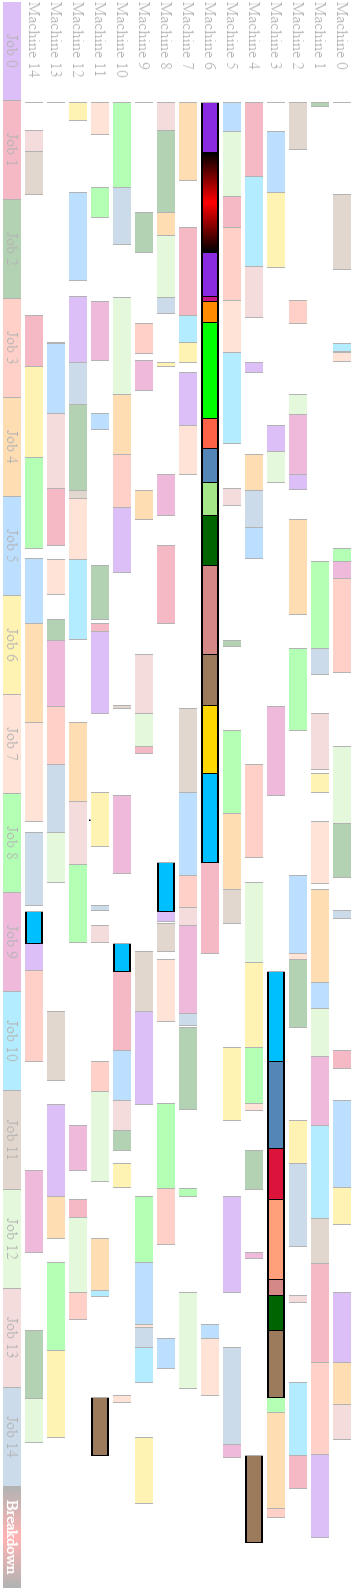
\includegraphics[scale=0.52]{rysunki/scheduleTail00.png}
\caption{Wygenerowany za pomocą napisanej biblioteki diagram Gantta.}{Czarno-czerwonym gradientem zaznaczono moment awarii maszyny 6.}
\label{rys_Gantt_HTML}
\end{center}
\end{figure}
%
\section{Parametryzacja i środowisko testowe}
Testy zostały przeprowadzone na laptopie z procesorem Intel Core i5 1.9GHz, 4GB pamięci RAM, na systemie Windows 10. Aplikacja realizująca opisane algorytmy została napisana w C++.\\\\
Kod wytworzony przez bibliotekę generującą HTML przetestowano na przeglądarce Google Chrome.\\\\
W algorytmie \emph{TSAB} przyjęto:
\begin{itemize}
 	\item długość listy tabu: 7,
 	\item długość listy najlepszych rozwiązań: 5,
 	\item $maxIter = 10$.
\end{itemize}
%
\section{Statystyki}
Uzyskane wyniki zestawiono w tabelach \ref{tab_res_one}, \ref{tab_res_two}, \ref{tab_res_three} oraz zaprezentowano na wykresach przedstawionych na rysunkach \ref{rys_wykres_czas_iID}, \ref{rys_wykres_czas_FonCP}, \ref{rys_wykres_cmax_iID}. Oznaczenia, jakie przyjęto:
\begin{itemize}
	\item $\mathbf{iID}$ -- unikalny identyfikator badanej instancji.
	\item $\mathbf{totNOper}$ -- jak poprzenio, całkowita liczba operacji w harmonogramie.
	\item $\mathbf{t_{AVG}}$ -- średni czas obliczeń algorytmu (w sekundach); mniej = lepiej.
	\item $\mathbf{\underline{C_{max}}}$ -- najmniejszy uzyskany $C_{max}$.
	\item $\mathbf{\overline{C_{max}}}$ -- największy uzyskany $C_{max}$.
	\item $\mathbf{F_{onCP}}$ -- jak często awaria miała wpływ na wydłużenie harmonogramu/znajdowała się na ścieżce krytycznej (wartość znormalizowana); mniej = lepiej.
\end{itemize}
\begin{table}[ht]
\renewcommand{\arraystretch}{1.2}
% 0 start
\begin{tabularx}{\textwidth}{|X|c|c|c|c|c|c|c|c|c|c|}
\hline
$\mathbf{iID}$ & \textbf{ta00} & \textbf{ta01} & \textbf{ta02} & \textbf{ta03} & \textbf{ta04} & \textbf{ta05} & \textbf{ta06} & \textbf{ta07} & \textbf{ta08} & \textbf{ta09}\\
\hline
$\mathbf{totNOper}$ & 225 & 225 & 225 & 225 & 225 & 225 & 225 & 225 & 225 & 225\\
\hline
$\mathbf{t_{AVG}}$ & 0.79 & 1.05 & 1.42 & 1.48 & 1.46 & 1.06 & 1.15 & 1.49 & 1.37 & 1.23\\
\hline
$\mathbf{\underline{C_{max}}}$ & 1441 & 1377 & 1376 & 1452 & 1505 & 1383 & 1310 & 1340 & 1467 & 1407\\
\hline
$\mathbf{\overline{C_{max}}}$ & 1486 & 1407 & 1467 & 1531 & 1632 & 1484 & 1482 & 1398 & 1482 & 1479\\
\hline
$\mathbf{F_{onCP}}$ & 1.00 & 0.40 & 1.00 & 1.00 & 1.00 & 1.00 & 1.00 & 1.00 & 0.00 & 1.00\\
\hline
%\end{tabularx}
% 0end
% 1 start
%\begin{tabularx}{\textwidth}{|X|c|c|c|c|c|c|c|c|c|c|}
\hline
$\mathbf{iID}$ & \textbf{ta10} & \textbf{ta11} & \textbf{ta12} & \textbf{ta13} & \textbf{ta14} & \textbf{ta15} & \textbf{ta16} & \textbf{ta17} & \textbf{ta18} & \textbf{ta19}\\
\hline
$\mathbf{totNOper}$ & 300 & 300 & 300 & 300 & 300 & 300 & 300 & 300 & 300 & 300\\
\hline
$\mathbf{t_{AVG}}$ & 2.33 & 2.31 & 1.59 & 2.29 & 1.99 & 1.58 & 2.09 & 1.37 & 1.80 & 2.97\\
\hline
$\mathbf{\underline{C_{max}}}$ & 1611 & 1577 & 1581 & 1597 & 1589 & 1551 & 1653 & 1669 & 1570 & 1584\\
\hline
$\mathbf{\overline{C_{max}}}$ & 1702 & 1701 & 1671 & 1668 & 1681 & 1618 & 1782 & 1745 & 1653 & 1657\\
\hline
$\mathbf{F_{onCP}}$ & 0.40 & 0.20 & 1.00 & 1.00 & 0.20 & 1.00 & 1.00 & 1.00 & 1.00 & 0.60\\
\hline
\end{tabularx}
% 1end
\caption{Część 1. Statystyki po 5 uruchomieniach aplikacji. W każdym przypadku awaria nastąpiła w chwili czasu 50 na maszynie nr 6. i trwała 100 jednostek czasu.}
\label{tab_res_one}
\renewcommand{\arraystretch}{1.0}
\end{table}
%
\begin{table}[!ht]
\renewcommand{\arraystretch}{1.2}
% 2 start
\begin{tabularx}{\textwidth}{|X|c|c|c|c|c|c|c|c|c|c|}
\hline
$\mathbf{iID}$ & \textbf{ta20} & \textbf{ta21} & \textbf{ta22} & \textbf{ta23} & \textbf{ta24} & \textbf{ta25} & \textbf{ta26} & \textbf{ta27} & \textbf{ta28} & \textbf{ta29}\\
\hline
$\mathbf{totNOper}$ & 400 & 400 & 400 & 400 & 400 & 400 & 400 & 400 & 400 & 400\\
\hline
$\mathbf{t_{AVG}}$ & 3.17 & 2.98 & 3.69 & 3.17 & 4.22 & 3.35 & 2.45 & 4.34 & 2.99 & 5.31\\
\hline
$\mathbf{\underline{C_{max}}}$ & 1921 & 1880 & 1803 & 1896 & 1880 & 1930 & 2062 & 1896 & 1831 & 1803\\
\hline
$\mathbf{\overline{C_{max}}}$ & 2014 & 1933 & 1850 & 1972 & 1961 & 2072 & 2180 & 2037 & 1982 & 1956\\
\hline
$\mathbf{F_{onCP}}$ & 1.00 & 1.00 & 1.00 & 0.00 & 1.00 & 0.20 & 0.20 & 1.00 & 0.00 & 0.60\\
\hline
%\end{tabularx}
% 2end
% 3 start
%\begin{tabularx}{\textwidth}{|X|c|c|c|c|c|c|c|c|c|c|}
\hline
$\mathbf{iID}$ & \textbf{ta30} & \textbf{ta31} & \textbf{ta32} & \textbf{ta33} & \textbf{ta34} & \textbf{ta35} & \textbf{ta36} & \textbf{ta37} & \textbf{ta38} & \textbf{ta39}\\
\hline
$\mathbf{totNOper}$ & 450 & 450 & 450 & 450 & 450 & 450 & 450 & 450 & 450 & 450\\
\hline
$\mathbf{t_{AVG}}$ & 1.20 & 1.90 & 1.37 & 1.92 & 1.34 & 2.22 & 2.37 & 3.30 & 2.16 & 3.01\\
\hline
$\mathbf{\underline{C_{max}}}$ & 2103 & 2154 & 2248 & 2091 & 2281 & 2241 & 2085 & 2022 & 2198 & 1917\\
\hline
$\mathbf{\overline{C_{max}}}$ & 2193 & 2260 & 2289 & 2204 & 2339 & 2309 & 2195 & 2052 & 2292 & 2043\\
\hline
$\mathbf{F_{onCP}}$ & 1.00 & 1.00 & 1.00 & 1.00 & 1.00 & 1.00 & 1.00 & 1.00 & 1.00 & 1.00\\
\hline
%\end{tabularx}
% 3end
% 4 start
%\begin{tabularx}{\textwidth}{|X|c|c|c|c|c|c|c|c|c|c|}
\hline
$\mathbf{iID}$ & \textbf{ta40} & \textbf{ta41} & \textbf{ta42} & \textbf{ta43} & \textbf{ta44} & \textbf{ta45} & \textbf{ta46} & \textbf{ta47} & \textbf{ta48} & \textbf{ta49}\\
\hline
$\mathbf{totNOper}$ & 600 & 600 & 600 & 600 & 600 & 600 & 600 & 600 & 600 & 600\\
\hline
$\mathbf{t_{AVG}}$ & 4.39 & 7.21 & 10.16 & 4.29 & 5.07 & 3.43 & 4.20 & 4.43 & 4.65 & 6.67\\
\hline
$\mathbf{\underline{C_{max}}}$ & 2443 & 2427 & 2326 & 2575 & 2368 & 2603 & 2379 & 2351 & 2364 & 2404\\
\hline
$\mathbf{\overline{C_{max}}}$ & 2565 & 2562 & 2415 & 2674 & 2456 & 2755 & 2480 & 2430 & 2424 & 2498\\
\hline
$\mathbf{F_{onCP}}$ & 1.00 & 1.00 & 1.00 & 1.00 & 1.00 & 0.80 & 1.00 & 1.00 & 1.00 & 1.00\\
\hline
%\end{tabularx}
% 4end
% 5 start
%\begin{tabularx}{\textwidth}{|X|c|c|c|c|c|c|c|c|c|c|}
\hline
$\mathbf{iID}$ & \textbf{ta50} & \textbf{ta51} & \textbf{ta52} & \textbf{ta53} & \textbf{ta54} & \textbf{ta55} & \textbf{ta56} & \textbf{ta57} & \textbf{ta58} & \textbf{ta59}\\
\hline
$\mathbf{totNOper}$ & 750 & 750 & 750 & 750 & 750 & 750 & 750 & 750 & 750 & 750\\
\hline
$\mathbf{t_{AVG}}$ & 2.71 & 2.61 & 2.33 & 1.85 & 3.19 & 2.66 & 2.35 & 1.65 & 3.04 & 2.00\\
\hline
$\mathbf{\underline{C_{max}}}$ & 3317 & 3275 & 2995 & 3121 & 3116 & 3140 & 3262 & 3395 & 2992 & 3004\\
\hline
$\mathbf{\overline{C_{max}}}$ & 3446 & 3388 & 3087 & 3237 & 3335 & 3283 & 3327 & 3511 & 3183 & 3058\\
\hline
$\mathbf{F_{onCP}}$ & 0.60 & 1.00 & 1.00 & 1.00 & 1.00 & 1.00 & 1.00 & 1.00 & 1.00 & 1.00\\
\hline
%\end{tabularx}
% 5end
% 6 start
%\begin{tabularx}{\textwidth}{|X|c|c|c|c|c|c|c|c|c|c|}
\hline
$\mathbf{iID}$ & \textbf{ta60} & \textbf{ta61} & \textbf{ta62} & \textbf{ta63} & \textbf{ta64} & \textbf{ta65} & \textbf{ta66} & \textbf{ta67} & \textbf{ta68} & \textbf{ta69}\\
\hline
$\mathbf{totNOper}$ & 1000 & 1000 & 1000 & 1000 & 1000 & 1000 & 1000 & 1000 & 1000 & 1000\\
\hline
$\mathbf{t_{AVG}}$ & 14.92 & 12.88 & 7.00 & 8.68 & 10.97 & 6.66 & 7.22 & 11.22 & 4.51 & 3.10\\
\hline
$\mathbf{\underline{C_{max}}}$ & 3191 & 3342 & 3157 & 3084 & 3153 & 3251 & 3303 & 3114 & 3515 & 3632\\
\hline
$\mathbf{\overline{C_{max}}}$ & 3296 & 3398 & 3294 & 3184 & 3257 & 3310 & 3528 & 3254 & 3589 & 3708\\
\hline
$\mathbf{F_{onCP}}$ & 1.00 & 1.00 & 1.00 & 1.00 & 1.00 & 1.00 & 1.00 & 1.00 & 1.00 & 1.00\\
\hline
%\end{tabularx}
% 6end
% 7 start
%\begin{tabularx}{\textwidth}{|X|c|c|c|c|c|c|c|c|c|c|}
\hline
$\mathbf{iID}$ & \textbf{ta70} & \textbf{ta71} & \textbf{ta72} & \textbf{ta73} & \textbf{ta74} & \textbf{ta75} & \textbf{ta76} & \textbf{ta77} & \textbf{ta78} & \textbf{ta79}\\
\hline
$\mathbf{totNOper}$ & 2000 & 2000 & 2000 & 2000 & 2000 & 2000 & 2000 & 2000 & 2000 & 2000\\
\hline
$\mathbf{t_{AVG}}$ & 10.01 & 10.53 & 7.23 & 8.75 & 11.03 & 12.18 & 11.67 & 7.60 & 12.11 & 5.82\\
\hline
$\mathbf{\underline{C_{max}}}$ & 6092 & 5575 & 6143 & 5627 & 6033 & 5797 & 5771 & 5831 & 5629 & 5706\\
\hline
$\mathbf{\overline{C_{max}}}$ & 6262 & 5740 & 6320 & 5727 & 6316 & 5981 & 5868 & 6055 & 5786 & 5838\\
\hline
$\mathbf{F_{onCP}}$ & 1.00 & 1.00 & 1.00 & 1.00 & 0.40 & 1.00 & 1.00 & 1.00 & 1.00 & 1.00\\
\hline
\end{tabularx}
% 7end
\caption{Część 2. Warunki jak podano w tabeli \ref{tab_res_one}.}
\label{tab_res_two}
\renewcommand{\arraystretch}{1.0}
\end{table}
%
\begin{figure}[h!]
\begin{center}
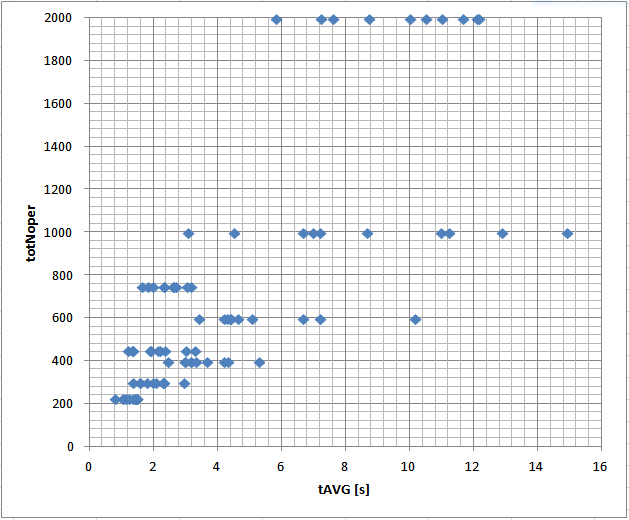
\includegraphics[scale=0.7]{rysunki/wykres_czas_iID.png}
\caption{Wykres przedstawiający średnie czasy wykonania algorytmu}{dla różnych rozmiarów instancji problemu gniazdowego.}
\label{rys_wykres_czas_iID}
\end{center}
\end{figure}
%
\begin{figure}[t!]
\begin{center}
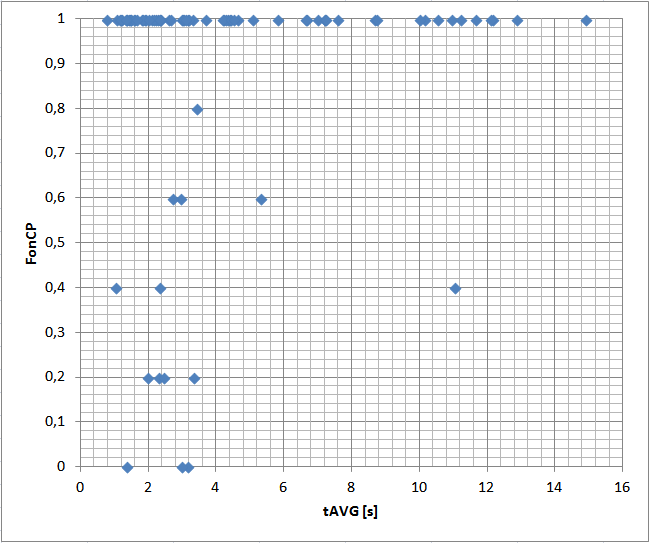
\includegraphics[scale=0.68]{rysunki/wykres_czas_FonCP.png}
\caption{Wykres przedstawiający znormalizowaną częstotliwość występowania}{awarii na ścieżce krytycznej dla różnych średnich czasów wykonania algorytmu.}
\label{rys_wykres_czas_FonCP}
\end{center}
\end{figure}
%
Z otrzymanych wyników można zauważyć, że średni czas obliczeń algorytmu jest wprost proporcjonalny do rozmiaru instancji. Oczywiście tak naprawdę czas ten jest zależny od rozwiązania, z którego startuje algorytm \emph{TSAB}, dlatego na wykresach zauważalny jest duży rozrzut tych czasów -- największy w przypadku instancji o rozmiarze 1000. Częstotliwość występowania awarii na ścieżce krytycznej w trakcie eksperymentów w większości przypadków wyniosła 100\% (na wykresach i w tabelach wartość 1.0). Powodem jest sztywność testowanych instancji -- przykłady podane przez Taillarda reprezentują klasyczne Problemy Gniazdowe, więc nie ma alternatywnych maszyn, na które można by przerzucić operacje z maszyny, która ulega awarii, tak jak miało to miejsce podczas testowania przypadku przedstawionego w tabeli \ref{tab_res_three}. Zróżnicowanie wartości $C_{max}$ jest spowodowane tym, że algorytm zatrzymuje się w lokalnych minimach. Mimo prób zwiększenia liczby iteracji nie udało się osiągnąć znacząco lepszych rezultatów. Również w tym przypadku, różnica $\overline{C{max}} - \underline{C{max}}$ jest wprost proporcjonalna do rozmiaru instancji, ale wzrost ten jest bardzo powolny -- do instancji o rozmiarze 1000 wydaje się wręcz, że utrzymuje się na stałym poziomie.
\begin{figure}[t!]
\begin{center}
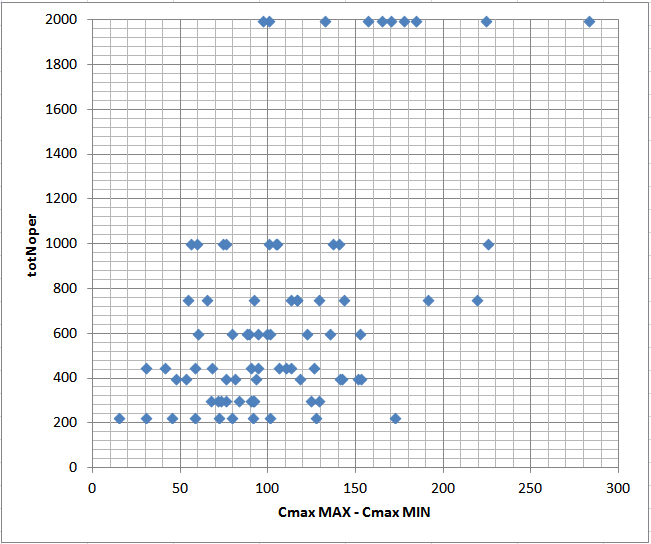
\includegraphics[scale=0.68]{rysunki/wykres_cmax_iID.png}
\caption{Wykres przedstawiający zróżnicowanie otrzymanych}{wartości $C_{max}$ w zależności od rozmiaru instancji.}
\label{rys_wykres_cmax_iID}
\end{center}
\end{figure}
%
\begin{table}[ht]
\begin{center}
\renewcommand{\arraystretch}{1.2}
\begin{tabular}{|c|c|}
\hline
$\mathbf{iID}$ & \textbf{ka00}\\
\hline
$\mathbf{t_{AVG}}$ & 0,09\\
\hline
$\mathbf{\underline{C_{max}}}$ & 15\\
\hline
$\mathbf{\overline{C_{max}}}$ & 22\\
\hline
$\mathbf{F_{onCP}}$ & 0,6\\
\hline
\end{tabular}
\caption{Część 3. Dla ostatniej instancji, awaria wystąpiła}{na maszynie nr 6. w chwili czasu 5 i trwała 10 jednostek czasu.}
\label{tab_res_three}
\renewcommand{\arraystretch}{1.0}
\end{center}
\end{table}
%

%
\clearpage
\addcontentsline{toc}{chapter}{Wnioski i uwagi}
\chapter*{Wnioski i uwagi}
Wszystkie postawione cele projektu zostały zrealizowane. W literaturze znaleziono wiele różnych nurtów ukierunkowanych na korygowanie harmonogramów. Spośród nich wybrano problem harmonogramowania odpornego dla Elastycznych Problemów Gniazdowych.\\\\
Zaproponowany algorytm jest hybrydą metody inicjującej populację początkową w Algorytmie Genetycznym zaproponowanym przez Al-Hinai oraz ElMekkawy w \cite{AEHGAFJS_ElMekkawy11} oraz bardzo efektywnego \emph{TSAB} Nowickiego i Smutnickiego \cite{Smutnicki96}. Połączenie te dało znakomite rezultaty wydajnościowe w porównaniu z Algorytmem Genetycznym z \cite{AEHGAFJS_ElMekkawy11}.\\\\
Aby łatwiej było prezentować wyniki eksperymentów stworzono narzędzie służące do graficznej prezentacji otrzymywanych w eksperymentach wyników -- diagramów Gantt'a harmonogramów zwracanych przez algorytm. W dodatku \ref{ch_code_snippets}dostępny jest kod biblioteki do wykorzystania w aplikacjach pisanych w C++.\\\\
Analiza wyników pokazała, że w przypadku klasycznych Problemów Gniazdowych, które w przeciwieństwie do Elastycznych Problemów Gniazdowych nie definiują alternatywnych maszyn, na których można by wykonywać zadania z maszyny, która uległa awarii, harmonogramowanie odporne nie ma zastosowania -- otrzymane harmonogramy po wystąpieniu awarii niemal zawsze są opóźniane ($F_{onCP}$ > 0).\\\\
W przyszłości można by rozszerzyć możliwe do wykonania ruchy (algorytm NSP) o zamianę operacji między maszynami, aby uzyskać jeszcze krótsze harmonogramy przy zachowaniu ich odporności na zmiany wynikające z awarii. Wtedy też, aby lepiej zbadać problem harmonogramowania odpornego, można by uelastycznić przykłady podane przez Taillard'a, zakładając że definiują one W Pełni Elastyczne Problemy Gniazdowe, tzn. każda operacja może zostać przetworzona przez dowolną maszynę, przy czym czas wykonania operacji na każdej z maszyn byłby jednakowy.\\\\
Wszystkie pliki źródłowe można znaleźć w repozytorium \url{https://github.com/kejn/job-shop-HGA/tree/tabuSearch/jobshop_HGA}.
% BIBLIOGRAFIA
\newpage
%\clearpage        % ALBO
\clearpage % JEŻELI WYPADNIE NA STRONIE PARZYSTEJ
\addcontentsline{toc}{chapter}{Bibliografia} %utworzenie w spisie treści pozycji Bibliografia
\bibliography{bibliografia} % wstawia bibliografię korzystając z pliku bibliografia.bib - dotyczy BibTeXa, jeżeli nie korzystamy z BibTeXa należy użyć otoczenia thebibliography
% DODATKI DO PRACY
\begin{appendices}
\chapter{Biblioteka do generowania HTML dla C++ \label{ch_code_snippets}}
%
\section{Interfejs \texttt{ContentHTML}}
\lstinputlisting[language=C++]{../inc/html/ContentHTML.h}
%
\section{Klasa \texttt{TextContentHTML.h}}
\lstinputlisting[language=C++]{../inc/html/TextContentHTML.h}
\lstinputlisting[language=C++]{../src/html/TextContentHTML.cpp}
%
\section{Klasa \texttt{TagContentHTML}}
\lstinputlisting[language=C++]{../inc/html/TagContentHTML.h}
\lstinputlisting[language=C++]{../src/html/TagContentHTML.cpp}
%
\section{Klasa \texttt{PageHTML}}
\lstinputlisting[language=C++]{../inc/html/PageHTML.h}
\lstinputlisting[language=C++]{../src/html/PageHTML.cpp}
%
\section{Style CSS}
\lstinputlisting{../res/css/gantt_styles.css}
\section{JavaScript}
\lstinputlisting{../res/js/hover_functions.js}
\end{appendices}
\clearpage
%opcjonalnie może się tu pojawić spis rysunków i tabel
\addcontentsline{toc}{chapter}{Spis rysunków} %utworzenie w spisie treści pozycji
\listoffigures
\clearpage
%\addcontentsline{toc}{chapter}{Spis rysunków} %utworzenie w spisie treści pozycji
\addcontentsline{toc}{chapter}{Spis tabel} %utworzenie w spisie treści pozycji
\listoftables
\end{document}

